\section{Conclusion}
The Standard Model of particle physics is the best theoretical framework so far to describe the nature around us. Although severely experimentally tested, this theory has it shortcomings and can not explain phenomena such as neutrino masses, dark matter, or dark energy. The top quark is the heaviest particle in the Standard Model leading to the believe that it has an enhanced sensitivity to various new particles and interactions suggested by beyond the Standard Model theories. The top quark decays almost exclusively to a \PW\ boson and a bottom quark with a very short lifetime making it escape from any bound states. This makes it possible to directly study the top quark properties by analysing its decay products. New physics phenomena are probed by measuring the production rate of top quarks for studying the $\PW\Ptop\Pbottom$ vertex as well as searching for interactions that are heavily suppressed in the Standard Model. 

The Large Hadron Collider is a top quark factory, producing a large number of events containing top quarks. At the proton collision points, experiments are placed to study the collisions. The search presented in this thesis is performed on data collected by the Compact Muon Solenoid experiment at a centre-of-mass energy of 13 \TeV, resulting in 35.9 \fbinv. 


Flavour changing neutral currents are forbidden at tree level and  highly suppressed at higher order in the Standard Model. However, many beyond the Standard Model theories enhance their probability. In this thesis, a search in three lepton final states is performed for the production of single top quarks via the \tZq\ vertex, with $\Pquark=\Pcharm, \Pup$, or the top quark pair processes where one of the top quarks decay through this vertex.  No significant deviation with respect to the predicted background is observed and upper limits at 95\% confidence level are placed. The observed (expected) upper limits at 95$\%$ confidence level  on the branching fractions of top quark decays are: ${\mathcal{B}}(t \rightarrow uZ) < 0.024\%$ ($0.015\%$) and ${\mathcal{B}}(t \rightarrow cZ) < 0.045\%$ (0.037$\%$), assuming one non-vanishing coupling at a time. A summary of the (observed) expected limits on the FCNC \tZq\ vertex is shown in \fig{fig:zoom}. 
\begin{figure}[htbp]
	\centering
	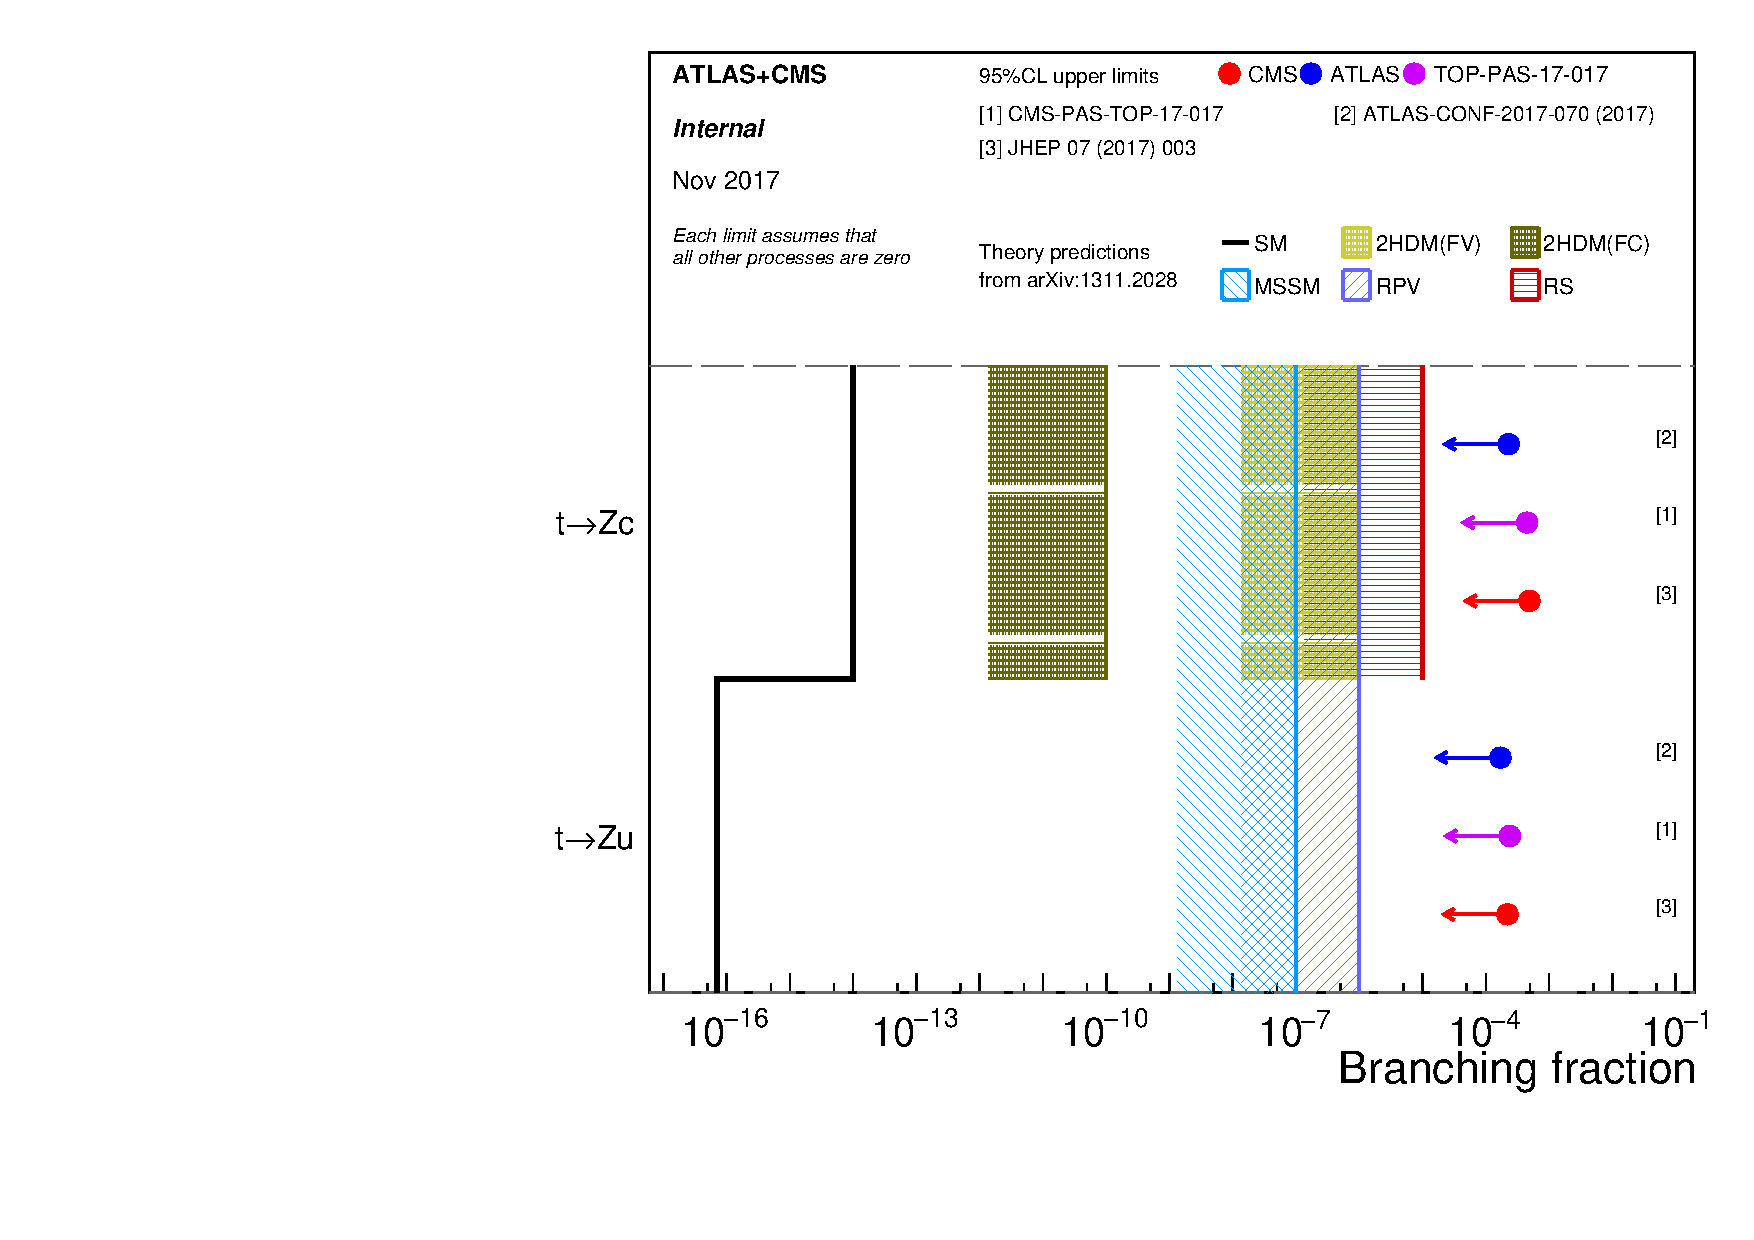
\includegraphics[width=0.49\linewidth]{7_Conclusion/Figures/fcnc_upperlimitszoom.pdf}
	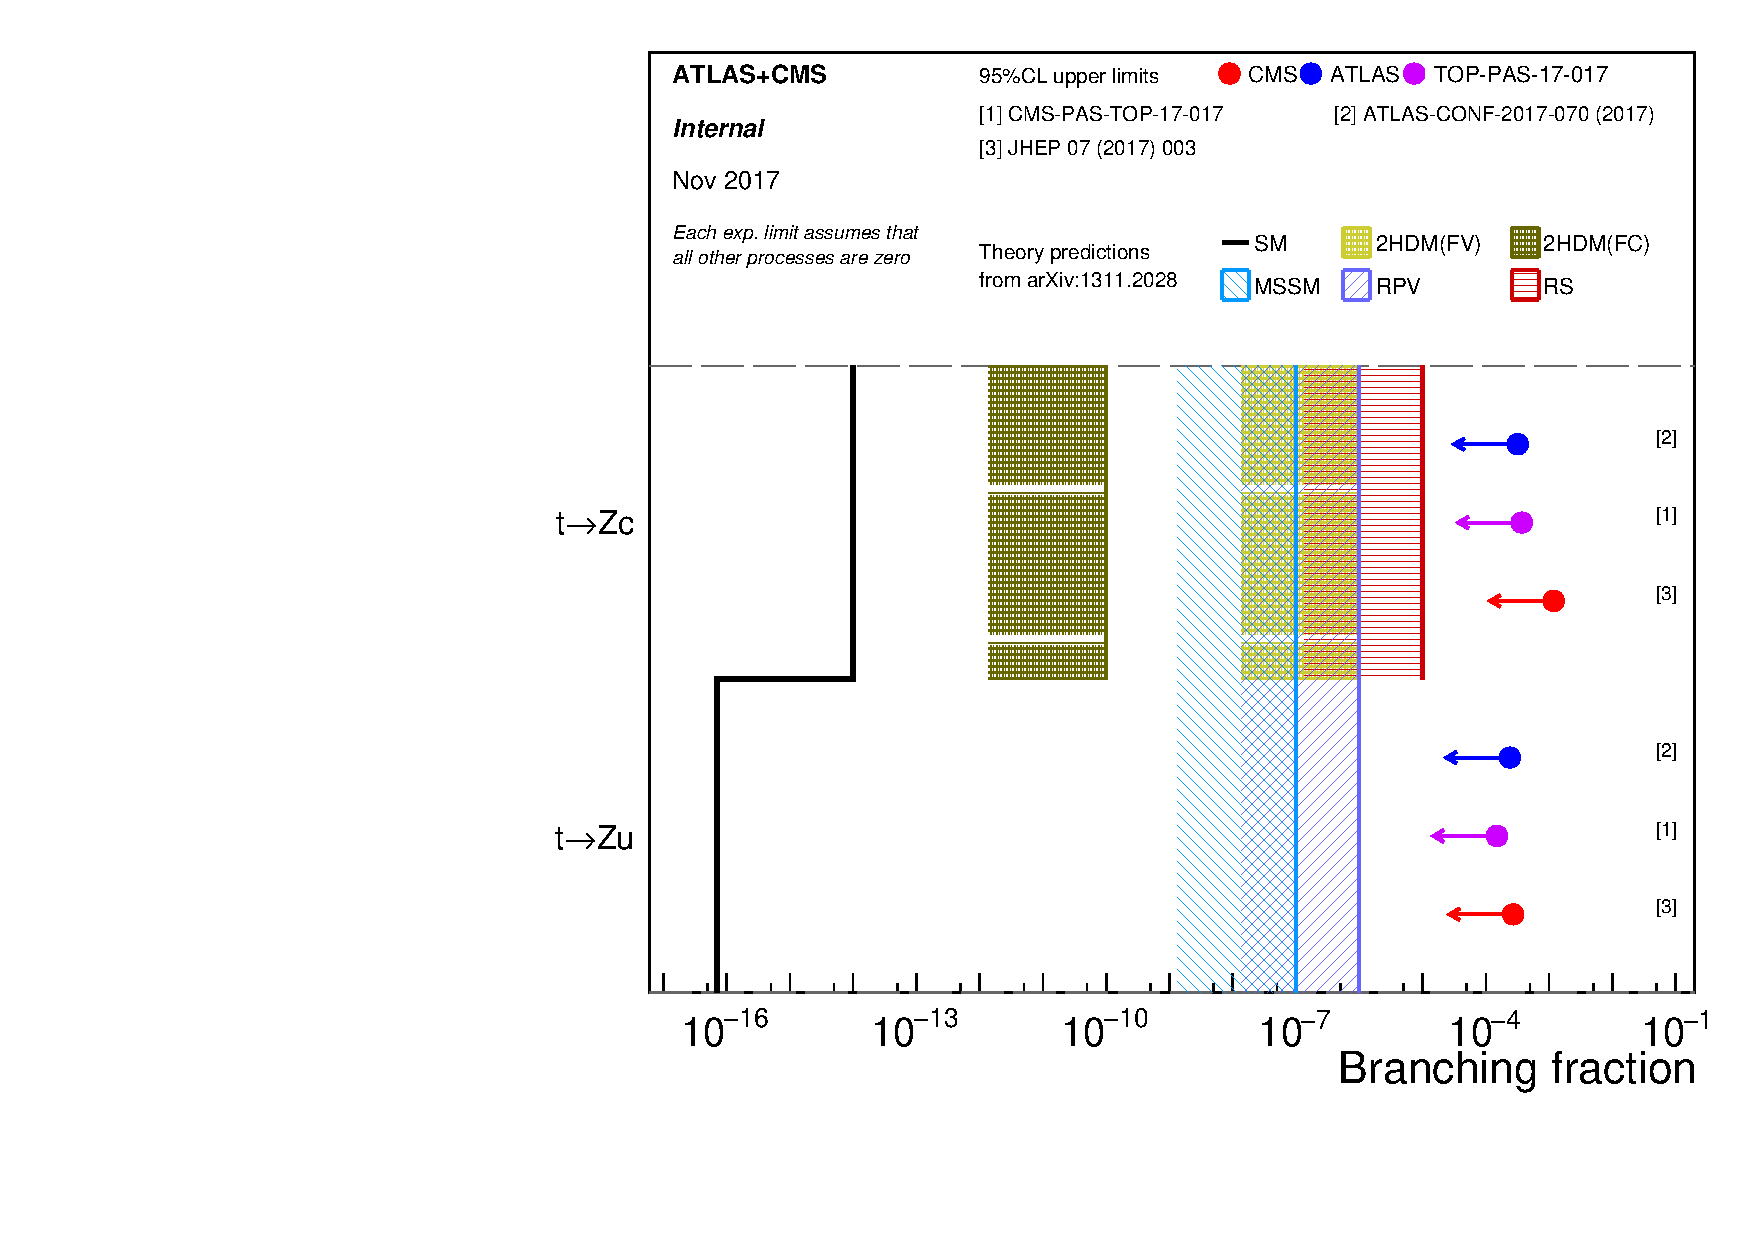
\includegraphics[width=0.49\linewidth]{7_Conclusion/Figures/fcnc_upperlimitszoomexp.pdf}
	\caption{Summary of the most stringent observed (left) and expected (right) upper limits on FCNC \tZq\ at 95\% CL upper limits from CMS (red) and ATLAS (blue) at a centre-of-mass of 8 and 13 \TeV. The results from this thesis are shown in purple. A comparison between theory predictions and experimental limits is shown. Figure adapted from \cite{summarywiki}.}
	\label{fig:zoom}
\end{figure}

Significant improvements are developed with respect to previous searches, namely by using other kinematic variables as input into the BDT as well as a better handle on the \NPL\ background.  The expected limit for the FCNC \Zut\ interaction is stronger than the current best observed (expected) limit of 0.017\% (0.024\%) set at a centre-of-mass energy of 13 \TeV\ by ATLAS~\cite{ATLAS-CONF-2017-070}.  The  observed (expected) limit on the \Zct\ interaction set by ATLAS is 0.023\% (0.032\%) and is comparable with the expected limit presented  in this search. In \fig{fig:fcncupperlimitss}, the branching fractions as predicted by the Standard Model and some beyond the Standard Model theories are presented together with the current most stringent limits. For the FCNC interactions with a \tZq\ vertex, the branching fractions predicted within the Standard Model or beyond the Standard Model theories are still out of reach. 
\begin{figure}[htbp]
	\centering
	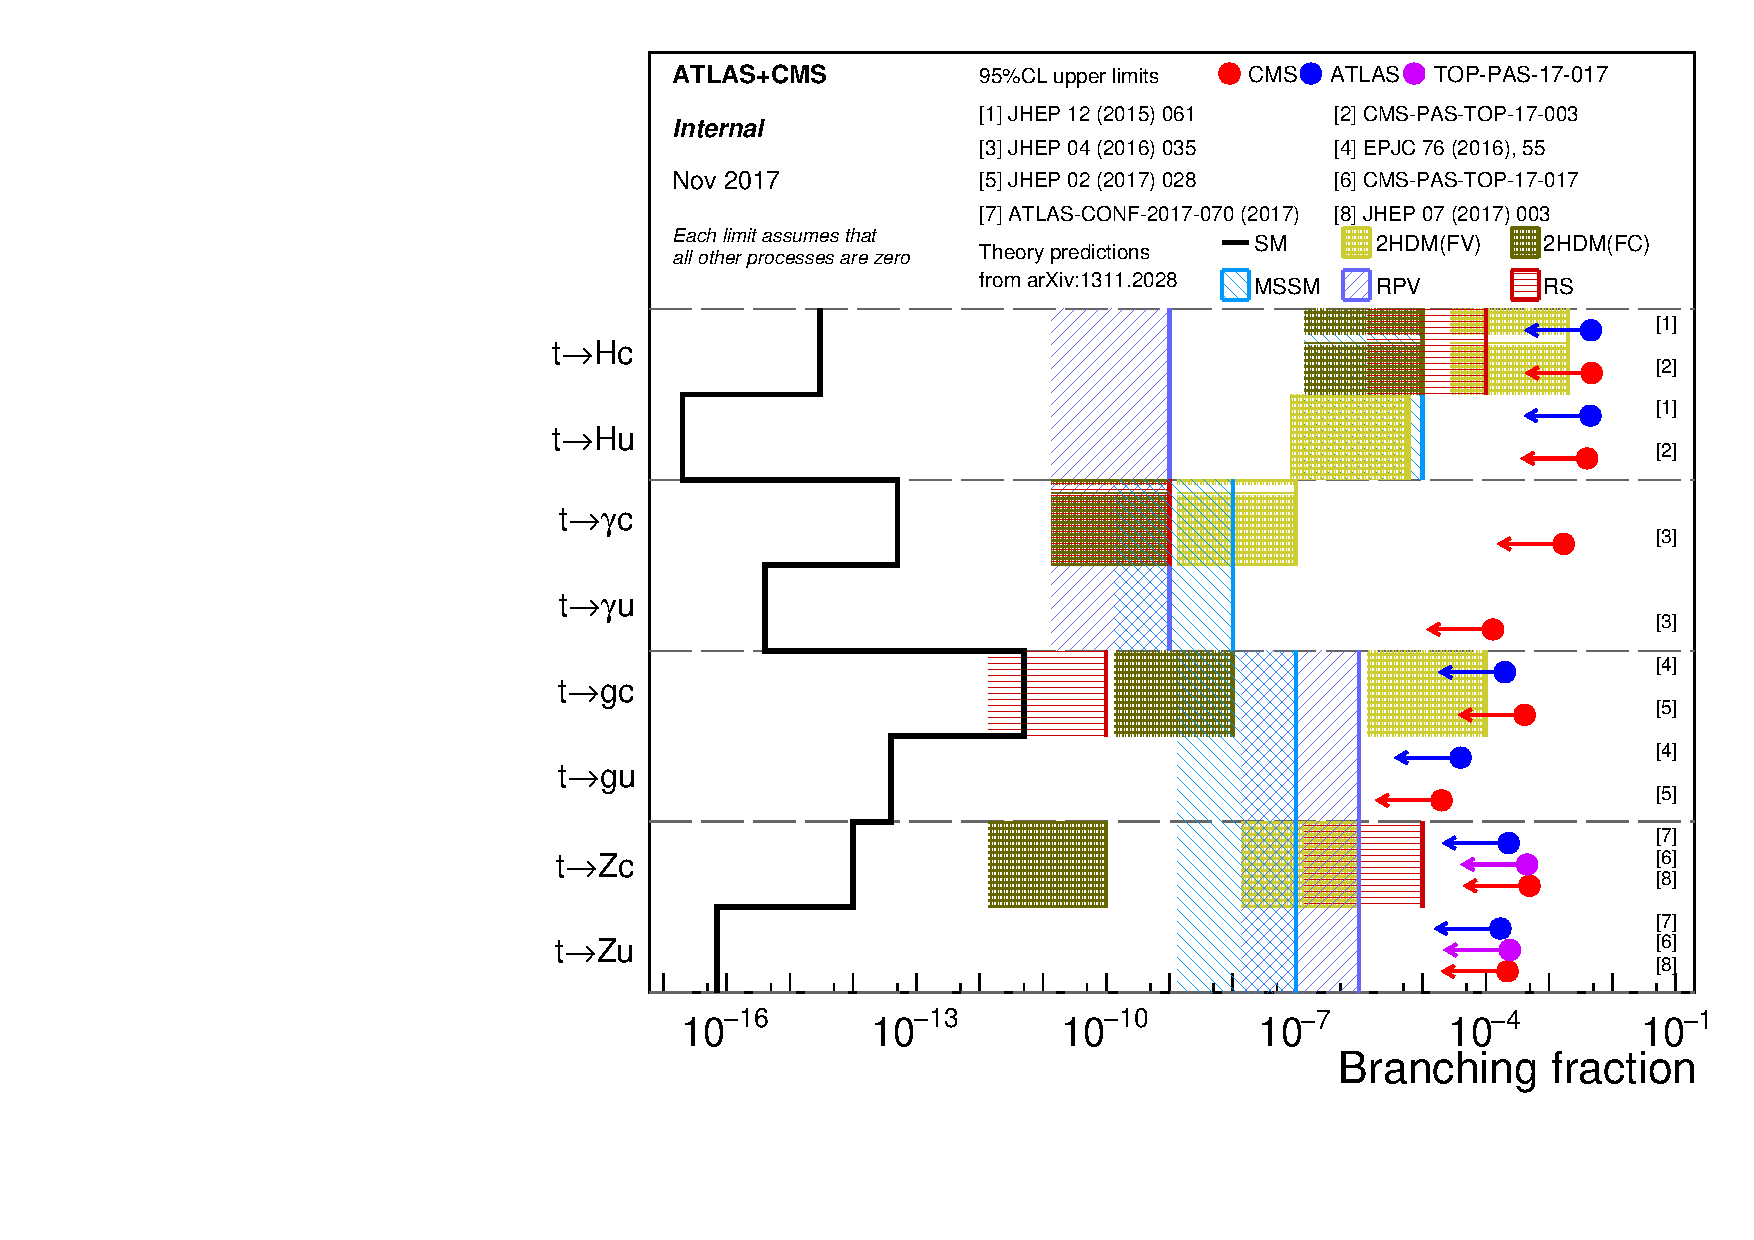
\includegraphics[width=0.7\linewidth]{7_Conclusion/Figures/fcnc_upperlimits.pdf}
	\caption{Summary of the most stringent upper limits on top-FCNC interactions at 95\% CL upper limits from CMS (red) and ATLAS (blue) at a centre-of-mass of 8 and 13 \TeV. The results from this thesis are shown in purple. A comparison between theory predictions and experimental limits is shown. Figure adapted from \cite{summarywiki}.}
	\label{fig:fcncupperlimitss}
\end{figure}


\clearpage
\section{Prospects}
\begin{figure}[htbp]
	\centering
	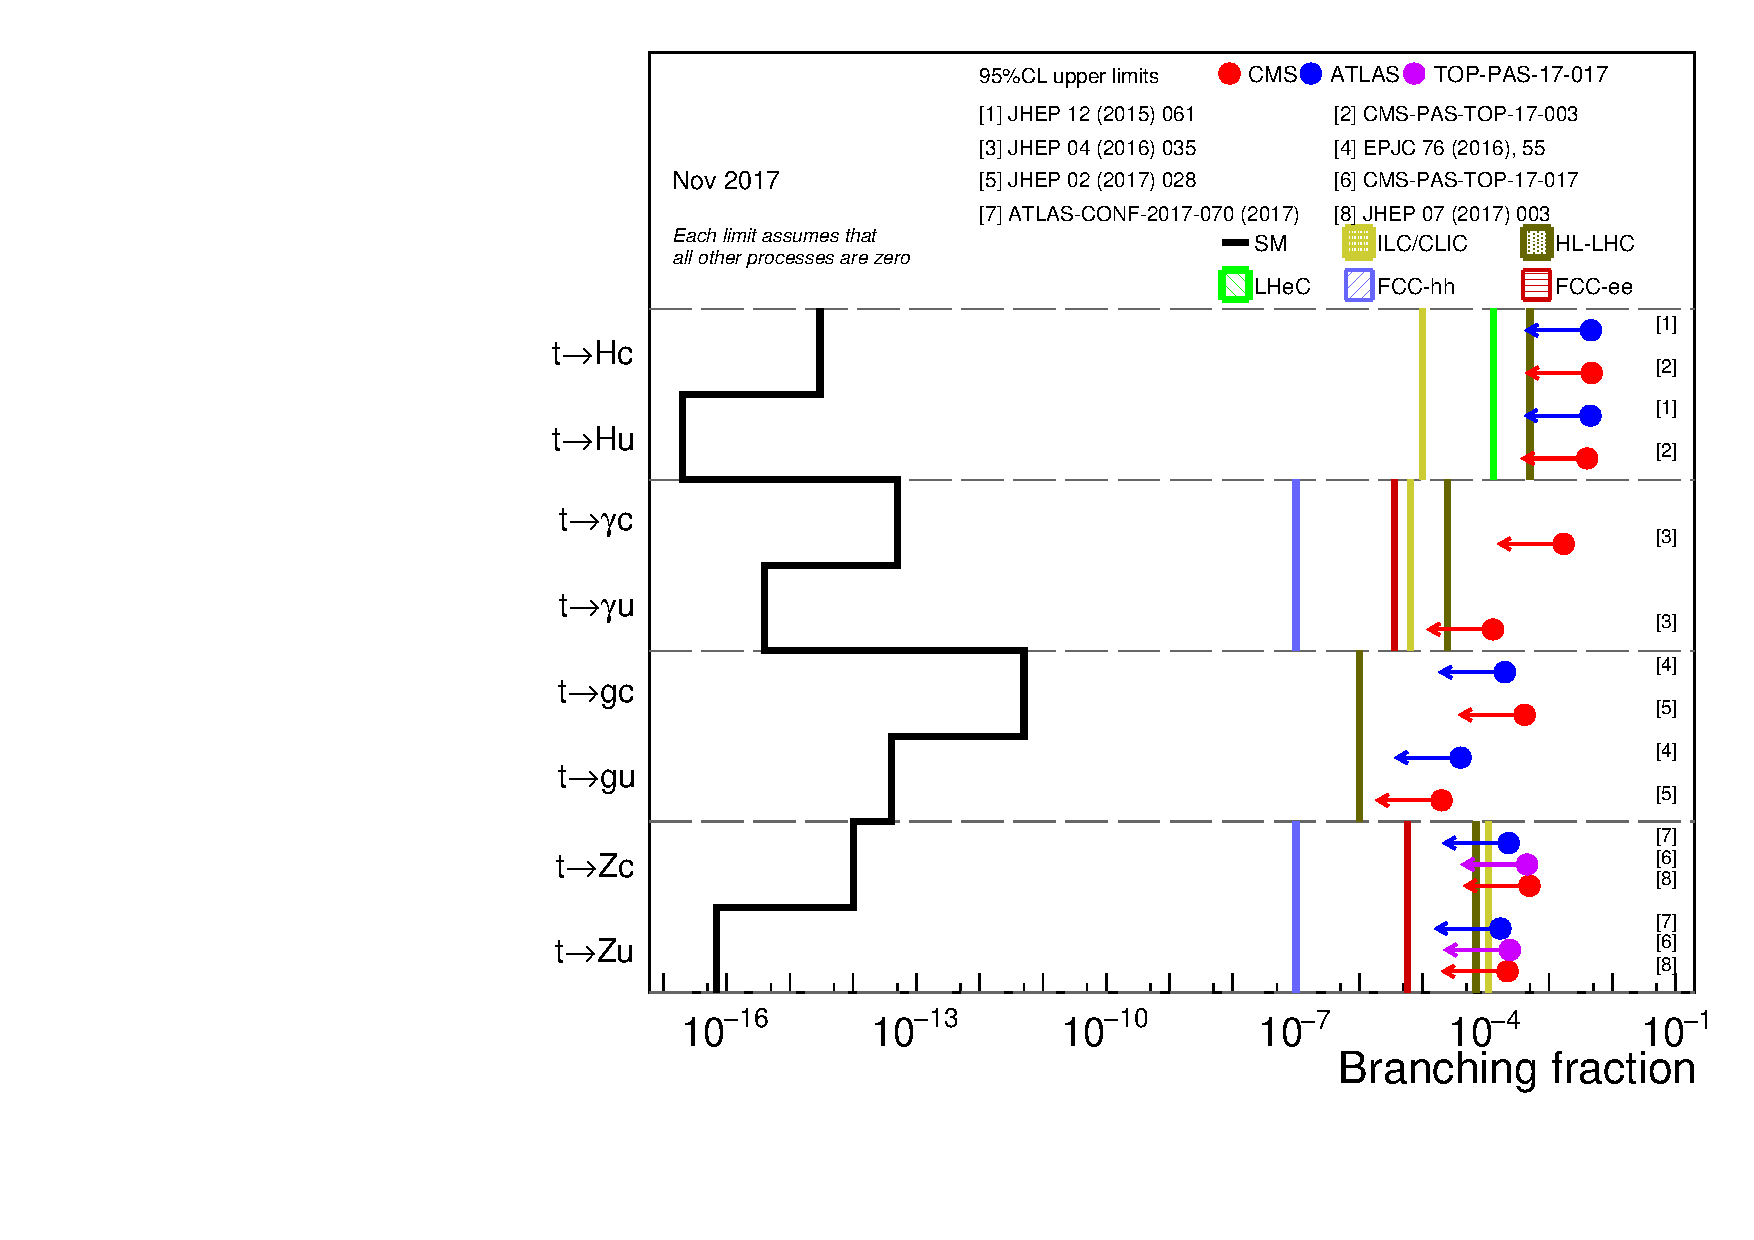
\includegraphics[width=0.7\linewidth]{7_Conclusion/Figures/fcnc_upperlimits_proj.pdf}
	\caption{Summary of the most stringent upper limits on top-FCNC interactions at 95\% CL upper limits from CMS (red) and ATLAS (blue) at a centre-of-mass of 8 and 13 \TeV. The results from this thesis are shown in purple. A comparison between the projections for future colliders and the current experimental limits is shown. Figure adapted from \cite{summarywiki}. The projections are taken from \cite{Liu:2015kkp,Agashe:2013hma,Khanpour:2014xla,Mangano:2016jyj}.}
	\label{fig:fcncupperlimitproj}
\end{figure}